\documentclass[12pt]{article}
\usepackage{graphicx}
\usepackage[hidelinks]{hyperref}
\usepackage{listings}
\usepackage{multicol}
\usepackage{caption}
\usepackage{listings,lstautogobble}
\usepackage{xcolor}

\usepackage{fontspec}
\setmainfont{Times New Roman}
\graphicspath{ {img/} }

\usepackage[a4paper, margin={0.7in, 0.7in}]{geometry}

\usepackage{fancyhdr}
\def\thetitle{Optical text transmission}
\pagestyle{fancy}
\fancyhead{}
\renewcommand{\headrulewidth}{0pt}
\fancyfoot[L]{Wrocław, 2024}
\fancyfoot[C]{\thetitle}
\fancyfoot[R]{\thepage}
\renewcommand{\footrulewidth}{0.5pt}

\definecolor{codegreen}{rgb}{0,0.6,0}
\definecolor{codegray}{rgb}{0.5,0.5,0.5}
\definecolor{codepurple}{rgb}{0.58,0,0.82}
\definecolor{backcolour}{rgb}{0.95,0.95,0.92}

\lstdefinestyle{CStyle}{
	backgroundcolor=\color{backcolour},   
	commentstyle=\color{codegreen},
	keywordstyle=\color{magenta},
	numberstyle=\tiny\color{codegray},
	stringstyle=\color{codepurple},
	basicstyle=\ttfamily\footnotesize,
	breakatwhitespace=false,         
	breaklines=true,                 
	captionpos=b,                    
	keepspaces=true,                 
	numbers=left,                    
	numbersep=5pt,                  
	showspaces=false,                
	showstringspaces=false,
	showtabs=false,                  
	tabsize=2,
	frame=single,
	language=C++
}

\newcommand{\image}[3]{
\begin{figure}[h]
	\begin{center}
		\includegraphics[scale=#3]{#2}
	\end{center}
  \caption{#1}
\end{figure}}

\usepackage{tocloft}
\renewcommand{\cftsecleader}{\cftdotfill{\cftdotsep}}

\begin{document}
	\begin{titlepage}
		\begin{center}
			
\includegraphics[scale=0.3]{img/pwr.png}\\
			\vspace{20pt}
			\textbf{Laboratory of Optoelectronics and Photonics} \\
			\textbf{Wrocław University of Science and Technology} \\
			\textbf{Chair of Electronic and Photonic Metrology}
			
			\vspace{20pt}
		
		\textbf{\huge\thetitle} \\
		\vspace{5pt}
		\Large Optoelectronics - project \\
		\vspace{20pt}
		\normalsize
		Group Number: \\
		
		\begin{tabular}{ |c|c|c| } 
			\hline
			Name & Surname & Album number \\ \hline
			Jakub & Kaszowski & 263544 \\ \hline
			Mikołaj & Pastucha & \\ \hline
			Fryderyk & Leszczyński & \\
			\hline
		\end{tabular} \\
		\vspace{5pt}
		Wrocław 2024 \\

		\end{center}
		
	\end{titlepage}	
  \newpage
	\tableofcontents{\thispagestyle{fancyplain}}
  \newpage
	
	\section{Introduction}
	% Subject of the report, content of the report
  The purpose of this project was to build a device capable of transmitting text using light. It should provide a Physical Layer for higher level arbitrary protocols.
  Such a device could be used in a variety of applications, such as remote control of any device that has a serial port.
  Any encoding could be used. Some of them could involve checksums and retransmission. Our device will however send a message in one direction, so even if the error is caught,
  there is no means to request a retransmission. Having in mind this assumption, we decided to use a morse code for encoding the information.
  This report elucidates a project that employs Morse code for intercommunication between two Printed Circuit Board (PCB) assemblies. The communication is facilitated by a light-emitting 
  diode (LED) transmitter and an LED receiver. The messages, originating from a computer terminal, are transmuted into Morse code, transmitted, received, and then demodulated back into alphanumeric characters for display.

  This report is a technical documentation of the project. It describes the initial assumptions, selected solutions and final result.
  It was developed during Optoelectronics course at Wrocław University of Science and Technology under supervision of dr. Daruisz Wysoczański.

	
	\section{Theoretical Introduction}
	% Domain, phenomena, methods, realizations, parameters, equations
 The project is situated within the realm of digital electronics and optical communication. It leverages the principle of optical transmission and reception of signals. The Morse code, a method of encoding text characters as standardized 
  sequences of two different signal durations, is used as the medium of communication. The hardware components employed include LEDs and STM32 microprocessors. The system's performance is contingent on parameters such as signal strength, 
  transmission distance, and ambient light interference. The mathematical model for the Morse code encoding and decoding process will be presented.
  Since the aim of the project is transmitting information using light, elements capable of transmitting and receiving light are needed
  They will be core parts of respectively a transmitter and receiver.
  \subsection{Transceiver}
  From available sources of light, we have decided to use a standard infrared diode used in any TV remote control. It can generate a light with wavelength of 940nm.
  Such diodes have many advantages and let us mitigate problems that we could have when using more sophisticated ligth source. One of our alternatives were lasers that
  can be found in our lab. The provide more directed and more intense light, but require power supply and the modulation of such light would be complex.
  The another factor for such choice is price and availability. The used infrared led was purchased at local electronic shop and is fairly inexpensive - costs less than 1\$.
  \begin{multicols}{2}
    \centering
    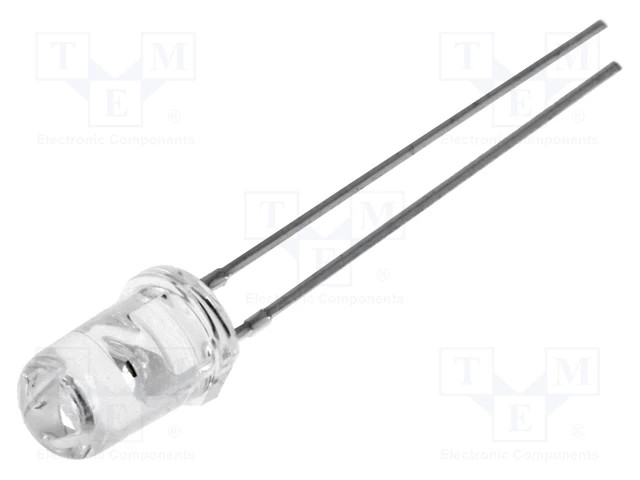
\includegraphics[scale=0.6]{ir_diode.jpg}
    \captionof{figure}{Infrared LED} \par
    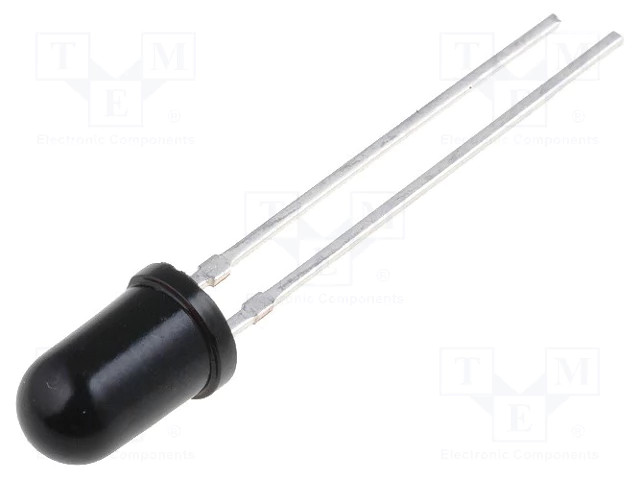
\includegraphics[scale=0.6]{photodiode.jpg}
    \captionof{figure}{Photodiode} 
\end{multicols}
  
  \subsection{Receiver}
  The crucial element of the setup is the sensing element measuring the light sent by transceiver.
  It should be chosen in such a way to maximise the useful signal and minimise the noise.
  A most common part used to measure light intensity in a hobbyist projects is a fotoresistor. Such element changes its resistance with the change of light conditions. 
  It can't be used in our device since it would be too prone to the interferences, as it has a wide sensing specturm.
  Since we decided to use a standard infrared diode, we chose to use a phototransistor made for the same light 
	
	\section{Assumptions}
	\subsection{Functional Assumptions}
	% What it does
  The system is architected to transmit alphanumeric messages from one terminal to another using Morse code as the communication protocol. The user inputs a message into the transmitting terminal. This message is then encoded into Morse code and 
  transmitted via the LED transmitter. The LED receiver picks up the transmitted Morse code signal, decodes it back into alphanumeric characters, and displays it on the terminal screen.
  The transmitter should be able to broadcast a message encoded as a morse code. It should take the input data from a serial port that should be easy to connect to a standard PC without specialized converter.
  The device should take a text message, turn in into a morse code and transmit.
  The receiver should listen continuously wait for any message to come. When it arrives, it should decode it into a useful form - back into a human readable text. In case a timing error happens, the user should be notified.
  Both of them should be easy to carry. Moreover they should be powered from a USB port with maximum current of 500mA.
  The functional requirements can be summarized as follows:
  \begin{itemize}
    \item Provide USB interface for sending/receiving data.
    \item Encode a message with morse code.
    \item Send and receive morse code.
    \item Decode morse code into a useful form.
    \item Detect idle line or incorrect timings.
    \item Does not need external power supply.
  \end{itemize}
	\subsection{Design Assumptions}
	% Method of implementing functional assumptions
  The system is implemented on the Arduino Black Pill platform, powered by STM32 microprocessors. The firmware, written in C, provides low-level control over the hardware peripherals and system resources. The design assumes a certain level of 
  proficiency in digital electronics, embedded systems, and C programming. The firmware handles tasks such as Morse code encoding/decoding, signal transmission/reception, and user interface management.
  We want our design to be easy to make at home. Thus, inexpensive off the shelf components are used.
  Also, the setup does not have a custom PCB - this makes it easy to reproduce for everyone, even using a breadboard.	
  The case is optional for the device operation. In our case it will be 3D printed.
  Our design should meet the following criteria:
  \begin{itemize}
    \item Off the shelf components are used.
    \item The costs should be minimized.
    \item The source code should be open source.
    \item The case is 3D printed.
  \end{itemize}
	\section{Description of the Hardware Part}
	% Block diagram + description
	% Photo of the actual system with reference to the block diagram
	% Mechanical part
	% Electrical schematics diagram + description
	% Key elements - descripion
	% PCBs, assembly diagram
	
	\section{Description of the Software}
	\section{Receiver software}
	% Main algorithm - diagram + description
	% Description of key functions (code examples)
	% Transmission protocols, key variables and parameters, etc.
	% Program listing in the appendices (with heading with the information about code type, hardware, author, version, date, etc.)
	% GUI - description
  The software on the microcontroller is responsible for following tasks:
  \begin{enumerate}
    \item Measure current signal level using builtin ADC.
    \item Quantize an analog signal into binary voltage levels.
    \item Continuously run converting algorightm.
    \item Recognize errors.
  \end{enumerate}

  \subsection{MCU selection}
  The selected MCU is STM32F411 that can be found onboard breakout module Blackpill. It contains USB periperial enabling us to communicate with serial emulators without a 
  dedicated USB to UART converter. It also has a builtin ADC with configurable resolution (in our case it is set to 12 bits) that runs in a continuous mod) that runs in a continuous mode.
  Additionally, it is equipped with a Floating Point Unint which significantly increases performance while performing math operations.
  The alternative for STM microcontrollers could be Arduino. It is also used for simliar projects, however it comes with much lower capabilites at the same price - there is no builtin serial to USB converter.
  Moreover, the debugging is supported only on STM, which proved crucial during implementation.

  \subsection{Toolchain}
  The STM32 can be programmed using both C and C++. The ARM company provides fork of gcc for the Cortex M4 cores that are used in the Blackpill, which use C++ 17 standard.
  We have decided to use STM32CubeIDE. It is an Eclipse based IDE that comes with proper compiler and visual configurator of the peripherals and clock. 


  With the complexity of an Cortex M4 core, the manual configuration of every peripheral and clock using registers is pretty tedious and error prone. In order to write a portable
  code, the Hardware Abstraction Layer libraries from the manufacturer were used. They significantly speed up the process of writing hardware drivers and lets us focus
  on the algorithm and achieving requirements. Moreover, the graphical tool lets us generate appropriate code for setting proper settings of peripherals and clocks.
  A very useful feature of all arm microcontrollers is SysTick interrupt \cite{stm32reference}. It is called each millisecond and increments a time variable.
  It enables us to measure time easily, without setting up a dedicated timer.

  \subsection{Analog to Digital Conversion}
  The selected microcontroller has a powerful successive approximation analog-to-digital converter onboard, capable of achieving 12 bits resolution.
  It can run in a single or continuous mode and optionally generate a DMA request to offload main CPU.


  In our case we use a single measurement mode. It means that each time that we want to get the value of analog voltage in digital form, we have to request it and wait for the event.
  It is suitable in our case because of low timing requirements. Our algorithm should work in such a way that a human operator could see the transmission and understand it.
  The timings of the ADC converter are shown below:
  
  \image{ADC timing diagram.}{adc_internals.png}{0.4}
  By setting the SWSTART bit, we can trigger a start a conversion process. Once it finishes, the End Of Conversion (EOC) bit is set.
  This process takes usually 15 clock cycles of ADC, which in our case is a few MHz.

  \subsection{Converting algorithm}
  The converting algorithm uses a preconfigured timing constraints that include times of: dash, dot, space between two signs, space between two letters, space between two words, timeout.
  \vspace{10pt}

  The main flow of the algorithm consists of following steps:
  \begin{enumerate}
    \item Calibrate reference value.
    \item Wait for start of transmission.
    \item Get chain of dash, dot and space.
    \item Analyze the chain and present human readable form.
  \end{enumerate}
  The schematic of the algorithm looks as follows:
  \image{Algorithm of the receiver.}{algorithm_receiver.png}{0.4}

  At the beginning, the code performs a calibration. It should establish a reference value of an environmental noise.
  When finished, the algorithm enters idle state. Here it waits for a transmission to start. It continuously measures the input value and waits for the high state.

  Once the transmission has started, it can measure the length of the high state. Next step is to compare measured value to predefined one and classify signal as a dash, dot or timing error.
  Following the high state, the low state is measured. If it is too long, the timeout is detected. The user is notified of an error and the algorithm
  returns to the idle state.

  The other possiblity is that the low state is measured to be a pause between signs, letters or words. If, it is noted as such and the code goes back to measuring high state to get the next sign.
  The listing of a full code can be found at the end of this report.

  \subsection{Error detection}
  The first method error detection is performed by comparing measured times to the expected values.
  The second method is analysis of the chain of dots and dashes. If it happens that the combination does not match any letter in the standard, a question mark is inserted.
  \begin{figure}
  \begin{lstlisting}[autogobble,style=CStyle]
  #include <iostream>
  std::array<int> ok;
  \end{lstlisting}
    \caption{Code responsible for morse code decoding. Unknown sequence return question mark.}
  \end{figure}
	
	\section{Start-up, Calibration}
	% First start-up, calibration
  During the start-up, the calibration procedure is needed. It is impossible to know in what ligh conditions the device will operate, so the reference value of light intensity is not hardcoded.
  Instead, a short procedure is executed at each startup. It does not take more than 3 seconds which is usually negligeble since the operator won't even have time to open serial connection in this time.
	
	\section{Test Measurements}
	% Measurement conditions
	% Compilation and interpretation of results
	% Definition of parameters: Full specification of the device/system.
	
	\section{User Manual}
	% Independent part, no reference to other projects of the report, possible repetition of figures, etc. Independent numbering of figures, tables, equations
	
	\section{Summary}
	% Work subject, results achieved, encountered problems, visions for the future
  As a result, two separate devices were built. Both of them fullfill the initial assumptions.
  The transceiver gets data from serial port emulated in USB, encodes it as a morse code and transmits.
  The receiver perfroms calibration, classification of the current state of the line and performs algorithm for decdoing the morse code into the text message. It also detects and notifies user about timing errors.
	
	\begin{thebibliography}{9}
		% Bibliography
    \bibitem{stm32reference} STM32F412 Reference Manual - RM0402 (2020), \emph{ST Microelectronics}
	\end{thebibliography}
	

  \section*{Appendices}
	\appendix
	\section{Technical drawing of case}
	\section{Electrical schematic}
	\section{Full code listing}
	% Dimensioned patterns of PCBs
	% Full listing
	% Key fragments of catalog notes
	% Custom drawings
	
\end{document}
